% This section will introduce the main ideas and methods used in \ac{FTC}. Moving forward in this section, classification follows the layout presented in \cite{Zhang2008BibliographicalSystems}. Zhang categorizes \ac{FTC} methods up until 2008. Methods developed after 2008 will have their own reference. 


A closed-loop control system capable of accommodating actuator faults while retaining its performance capability is said to be a \textit{Fault-Tolerant Control System}. Such a system is critical in systems such as \ac{S/C} and nuclear facilities, among others. 

A \ac{FTCS} can be put in two main categories, \textbf{passive} and \textbf{active}. A \ac{PFTCS} uses a robust controller designed to handle a handful of pre-programmed failures. This method has a number of advantages; no \ac{FDD} is necessary since the controller never expects to know what has gone wrong, it simply observes a new sensor input and uses its robust control scheme to compensate. No controller reconfiguration including parameter recalculation and reconfiguration lag. This method is, however, limited in its ability to handle severe faults. In contrast, \ac{AFTCS}'s uses sensors to identify faults, reconfigure the control system in such a way as to use the remaining actuators as efficiently as possible. 
\todo[inline]{Analogy? really?}
Imagine you are driving home from work, and suddenly you hit a nail and puncture your tire. Lucky for you, you just installed new run-flat tires (tires that continue to work even when punctured, albeit with a reduced efficiency), allowing you to continue your drive at a slower speed. This is \ac{PFTCS}, the run-flat tire handled the fault and allowed the car to continue operation at a reduced pace. A \ac{AFTCS} could have used a pressure sensor in the tire to realize when the tire was punctured, and automatically deploy a tire repair kit. This way, you can continue driving the car with no problems. \todo{might be silly analogy..}

\subsection{FTC Structure}

The figure below \todo{Ill make my own figure} depicts the general structure for a \ac{AFTCS}. As we will see, different control systems vary greatly in block choices and structure. This figure should thus not be seen as an absolute but rather serve as a first principles visual aid. \todo{holy wording...} Some of the blocks in the figure (Actuators, Sensors, and System) \todo[fancyline]{fix with new figure} are not explicitly explain and will be explained in detail in later chapters. Some additional blocks are not in the figure, these blocks are not fundamental and are only explained in the text. \todo[fancyline]{real?}

\begin{figure}[H]
    \centering
    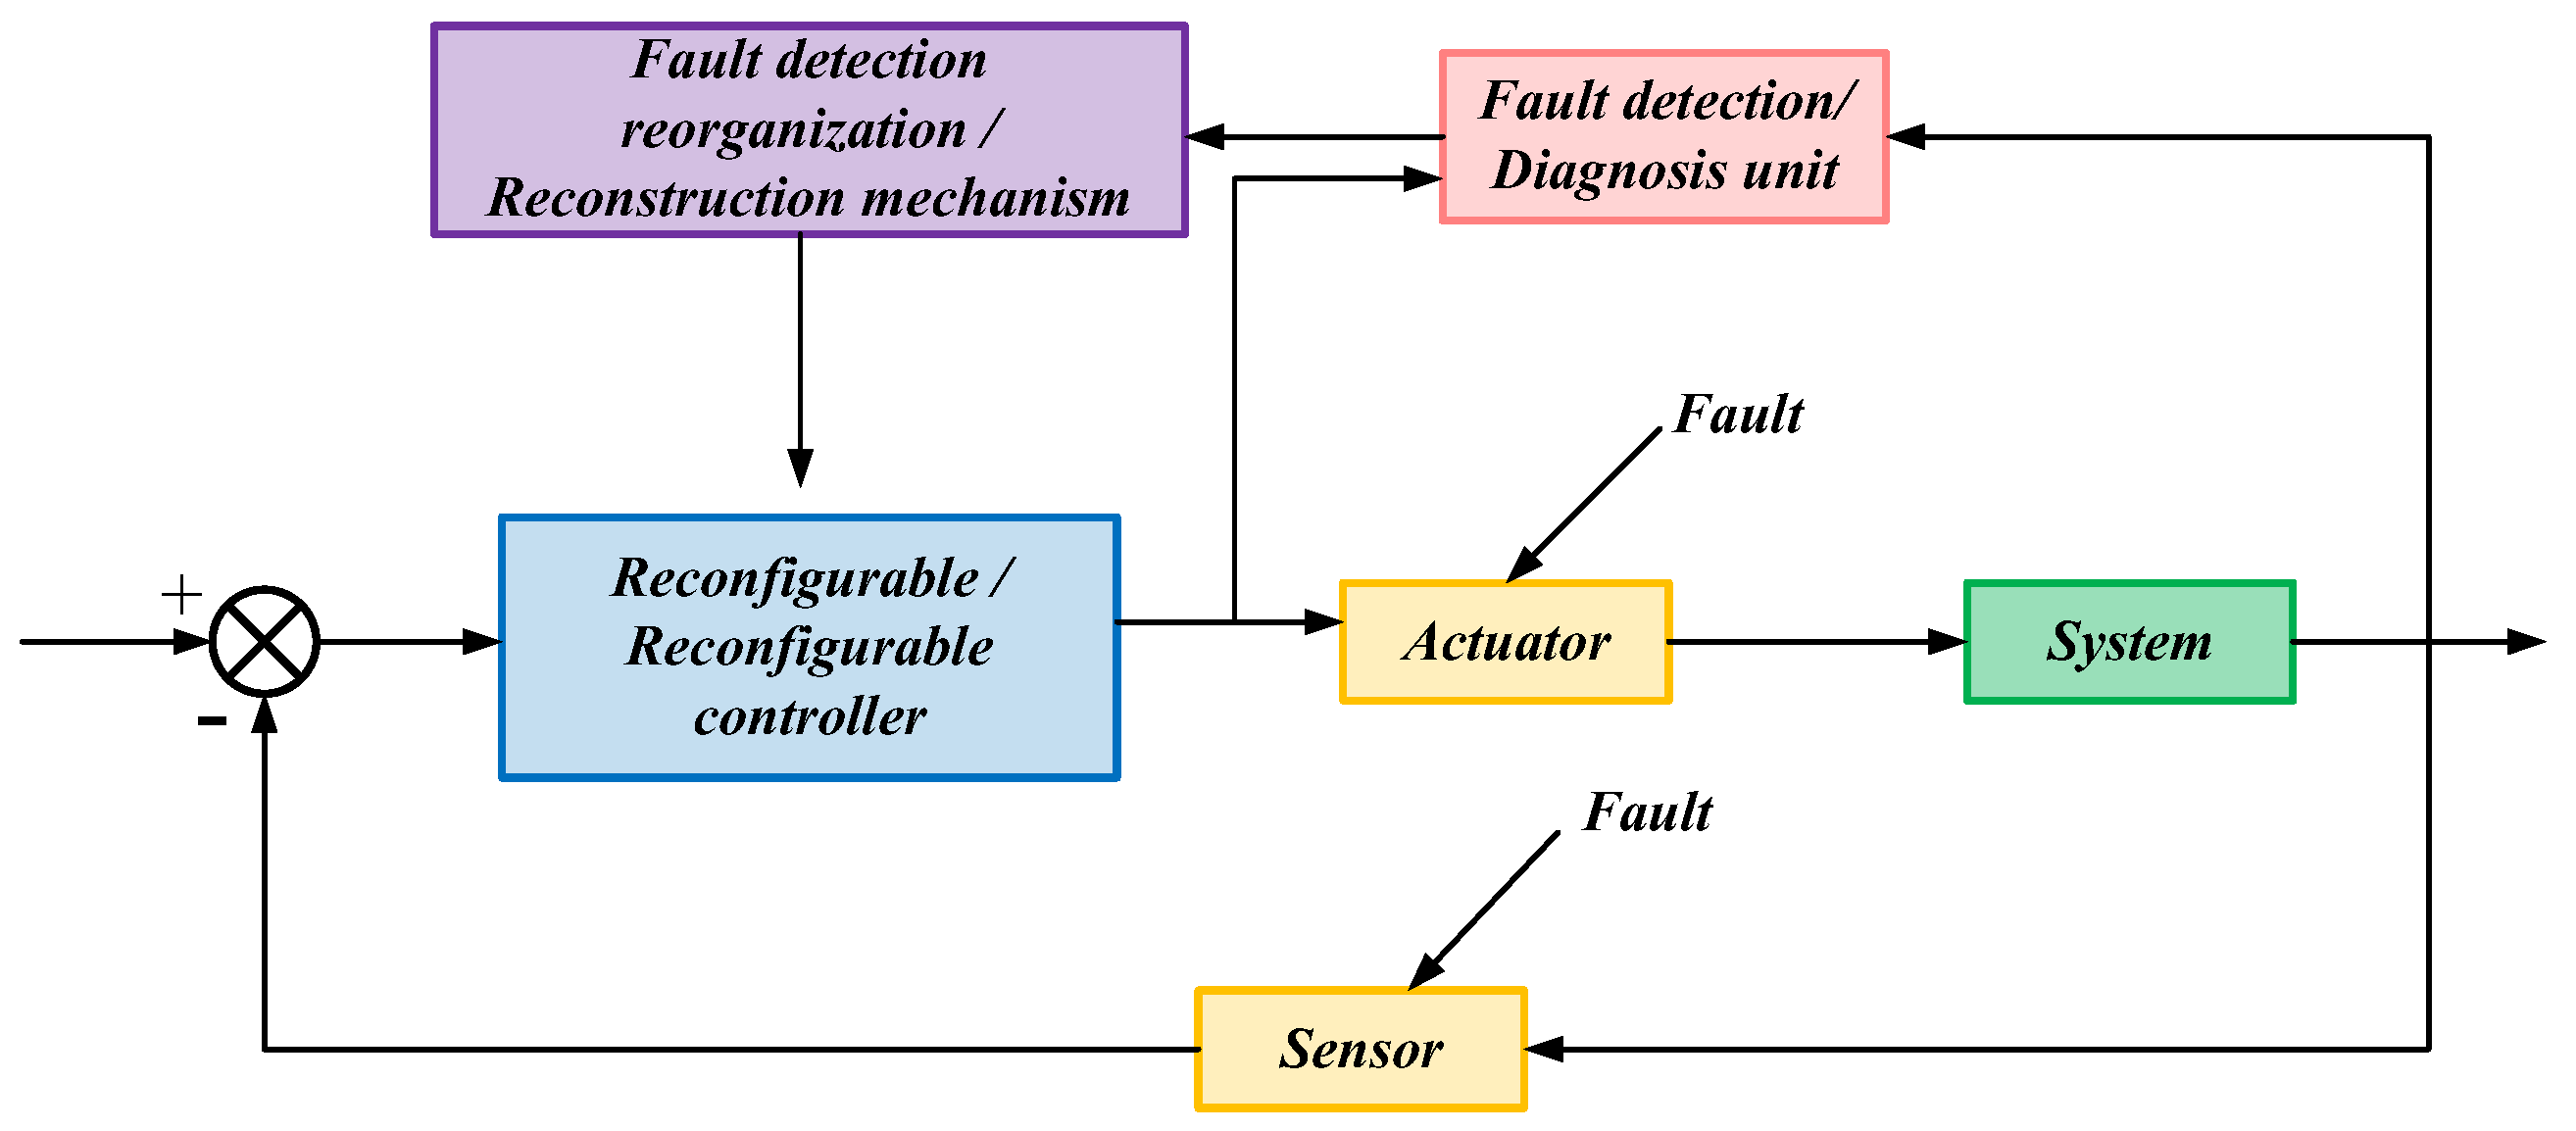
\includegraphics[width=0.5\linewidth]{images/basic_AFTCS.png}
    \caption{General structure of AFTCS}
    \label{fig:enter-label}
\end{figure}


\begin{itemize}

    \item \textbf{\ac{FDD} unit:} The \ac{FDD} could take inputs from various parts of the system depending on the design, but in general it takes signals outputted by the controller and compares them with the real-world effect.  This comparison can then lead to a conclusion on what has happened and report this to the \ac{RCU}.


    \item \textbf{\ac{RCU}:} This block listens to the \ac{FDD} unit for faults. Once a fault is detected, the \ac{RCU} reconfigures the controller to account for the new dynamics. The way the reconfiguration is performed can vary drastically and is part of what classifies the system as we will learn later.
    
    \item \textbf{Reconfigurable controller:} The reconfigurable controller acts as a normal controller during normal operations. Once the \ac{RCU} sends a reconfiguration request the controller will change in some way. As mentioned earlier, the way the controller change changer with design. 

    
    \item \textbf{Additional optional blocks (not in the figure \todo[fancyline]{or are they :) hmmmm}): } 
    \begin{itemize}
        \item \emph{\ac{CA}:} Usefull in over actuated systems where control effort can be redistributed over the functioning actuators. 

        \item \emph{Decision Layer:} Relatively new technique utilizing something like Behavior trees or \ac{NN} to orchestrate a multitude of strategies within a single system, switching to the most optimal strategy for the current situation.

        \item \emph{Reference/Command Governors:} filters that modify commands so they stay within actuator limits. In spacecraft FTC, they prevent saturation or instability after faults by slowing or reshaping reference signals without changing the controller.
    \end{itemize}

    
\end{itemize}

% \begin{itemize}
%     \item Definition and Taxonomy of FTC, importance in spacecraft systems.\\
%     A close-loop control system capable of accommodating actuator faults while retaining performance capability is said to be a \textit{Fault Tolerant Control System :) }
%     \item Active vs. Passive FTC:
%         \begin{itemize}
%             \item Active FTC relies on Fault Detection and Diagnosis (FDD) with controller reconfiguration.
%             \item Passive FTC uses fixed controllers designed to tolerate a range of faults.
%         \end{itemize}
%     \item System components: controller, FDD scheme, reconfiguration mechanism, command/reference governor.
%     \item Key references: Zhang \& Jiang (2008), Jiang \& Yu (2012), Yin et al. (2016).
% \end{itemize}